\documentclass[fleqn]{article}
\usepackage[margin=1in]{geometry}
\usepackage[nodisplayskipstretch]{setspace}
\usepackage{amsmath, nccmath, bm}
\usepackage{amssymb}
\usepackage{enumitem}
\usepackage{graphicx}
\usepackage{float}
\usepackage{listings}
\usepackage{hyperref}
\usepackage[svgnames]{xcolor}
\graphicspath{{./images}}

\hypersetup{
    colorlinks=true,
    linkcolor=black,
    filecolor=black,      
    urlcolor=blue
    }

\newcommand{\zerodisplayskip}{
	\setlength{\abovedisplayskip}{0pt}%
	\setlength{\belowdisplayskip}{0pt}%
	\setlength{\abovedisplayshortskip}{0pt}%
	\setlength{\belowdisplayshortskip}{0pt}%
	\setlength{\mathindent}{0pt}}
	
\definecolor{vgreen}{RGB}{104,180,104}
\definecolor{vblue}{RGB}{49,49,255}
\definecolor{vorange}{RGB}{255,143,102}

\lstdefinestyle{verilog-style}
{
    language=Verilog,
    basicstyle=\small\ttfamily,
    keywordstyle=\color{vblue},
    identifierstyle=\color{black},
    commentstyle=\color{vgreen},
    numbers=left,
    numberstyle=\tiny\color{black},
    numbersep=10pt,
    tabsize=8,
    moredelim=*[s][\colorIndex]{[}{]},
    literate=*{:}{:}1
}

\lstset{style={verilog-style},showstringspaces=false}

\makeatletter
\newcommand*\@lbracket{[}
\newcommand*\@rbracket{]}
\newcommand*\@colon{:}
\newcommand*\colorIndex{%
    \edef\@temp{\the\lst@token}%
    \ifx\@temp\@lbracket \color{black}%
    \else\ifx\@temp\@rbracket \color{black}%
    \else\ifx\@temp\@colon \color{black}%
    \else \color{vorange}%
    \fi\fi\fi
}
\makeatother

\newcommand{\code}[1]{%
	\colorbox{Gainsboro}{\texttt{#1}}%
}

\title{Homework 4}
\author{Owen Sowatzke}
\date{April 16, 2025}

\begin{document}

	\offinterlineskip
	\setlength{\lineskip}{12pt}
	\zerodisplayskip
	\maketitle
	
	\begin{enumerate}
		\item ~
		
			\begin{figure}[H]
				\centerline{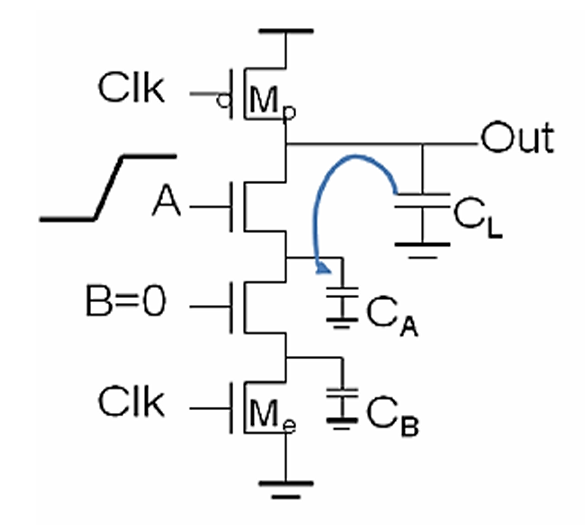
\includegraphics[width=0.5\textwidth]{circuit_question1.png}}
				\label{fig::circuit_question1}
			\end{figure}

			\begin{enumerate}
			\item[1.] Write out the output function in terms of A and B.			
			
			\begin{equation*}
				\mathbf{Out = \overline{AB}}
			\end{equation*}
			
			\item[2.] $V_DD=2.0\text{V}$, $|V_{th}|=0.6\text{V}$ for all PMOS and NMOS transistors. $C_L/C_A=3$, $C_L/C_B=5$; What is the voltage value at X and at output nodes ($V_x$ = ? and $V_{out}$ = ?)
			
			$V_{\text{out}}$ will be charged to $V_{DD}$ during the charge phase. Assume that all other nodes are charged to $0\text{V}$.
			
			When $A$ rises from 0 to 1. $C_L$ will discharge through $M_a$ and share charge with $C_A$. Because $B=0$, $M_b$ should be in the cutoff state, so there will be no charge sharing with $C_B$.
			
			Start by assuming that there is no voltage drop across $V_a$.
			
			\begin{equation*}
				C_LV_{DD} = (C_L + C_A)V_{out} 
			\end{equation*}			
			
			\begin{equation*}
				\Rightarrow V_x = V_{out} = \frac{C_LV_{DD}}{C_L + C_A} = \frac{3C_AV_{DD}}{3C_A + C_A} = \frac{3V_{DD}}{4} = 1.5\text{V}
			\end{equation*}
			
			 However, for $M_a$ to be on $V_{gs} < V_{th} \Rightarrow V_x \leq 1.4\text{V}$.
			
			Therefore, $V_x$ will charge to 1.4V, which will consume some of the charge in $C_L$.
			
			$Q_x = 1.4C_A$
			
			$\Rightarrow Q_{out} = C_LV_DD - Q_x = 2C_L - 1.4C_A = 6C_A - 1.4C_A = 4.6C_A$
			
			$\therefore V_\text{out} = Q_{out}/C_L = 4.6C_A/3C_A = \mathbf{1.53\text{\textbf{V}}},\ V_x = \mathbf{1.4\text{\textbf{V}}}$
			
			\end{enumerate}
			
		\item In the following figure, what king of logic is implemented in this circuit? Write out the Z function.
		
			\begin{figure}[H]
				\centerline{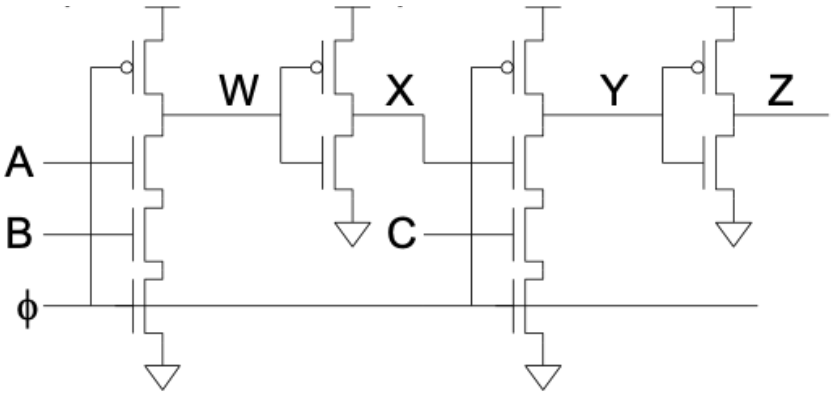
\includegraphics[width=0.5\textwidth]{circuit_question3.png}}
				\label{fig::circuit_question3}
			\end{figure}

			The dynamic logic gates implement the following equations:
			
			$W = \overline{AB}$
			
			$Y = \overline{XC}$
			
			The static CMOS gates implement the following equations:
			
			$X = \bar{W}$
			
			$Z = \bar{Y}$
			
			$\therefore$ Z can be computed as follows:
			
			$Z = \overline{\overline{XC}} = XC = \bar{W}C = \overline{\overline{AB}}C = \mathbf{ABC}$
			
			Alternatively, we can recognize Z as two chained domino AND gates.
			
			
	\end{enumerate}

\end{document}